\documentclass[10pt,times,twocolumn]{article}

\usepackage{sbcm2019}
\usepackage{graphicx,url}
\usepackage{hyperref}
\usepackage{tikz}
\usetikzlibrary{arrows.meta}
\usepackage{biblatex}
\addbibresource{example.bib}
\usepackage[table]{xcolor}
\usepackage{float}


\usepackage{booktabs} % Para líneas de tabla más profesionales
% -------------------------------------------------------
% Packages that facilitate double-blind peer review
% Comment the first line and uncomment the second to remove double-blindness
%\usepackage[blind]{anonymize} % Blind
\usepackage{anonymize} % not blind
% --------------------------------------------------------

%\usepackage[brazil]{babel}
%\usepackage[latin1]{inputenc}
% If needed, change this to:
\usepackage[utf8]{inputenc}
\usepackage[spanish]{babel}

\sloppy

\title{Análisis Funcional y Estructural de un Sistema de Gestión de Contenidos (CMS)}

\author
{
	\anonymize{Marco Acosta}\inst{1} 	
	\and
	\anonymize{Nilda Gómez}\inst{1}
	\and
	\anonymize{Nathaly Prieto}\inst{1}
	\and
	\anonymize{Elías Cristaldo}\inst{1}
}

\address{
	\anonymize{Ingeniería en Informática / 
	Facultad Politécnica / 
	Universidad Nacional de Asunción}\\
    \anonymize{Campus, San Lorenzo – Paraguay, Teléfono (+595-21) 588 7000}\\ \\
	\anonymize{\textit{23 de Junio del 2024\vspace{10pt}}}
}

\begin{document}

\maketitle

\begin{abstract}
Este artículo presenta una evaluación íntegra de la calidad del proyecto del Sistema de Gestión de Contenidos (CMS). El análisis de calidad es un componente fundamental en la ingeniería del software, garantizando que el producto satisfaga los estándares de eficiencia, seguridad, mantenibilidad y satisfacción del usuario, asegurando su confiabilidad y óptimo desempeño en diversas condiciones de uso \cite{swebok}. El proceso de evaluación se desglosa en tres etapas principales \cite{pressman}, la primera aborda la calidad de concordancia, evaluando el grado de cumplimiento de las especificaciones de diseño. La segunda etapa analiza la calidad del diseño, considerando la tolerancia a fallos y las especificaciones de rendimiento. La tercera y última etapa se centra en la calidad del software, examinando la conformidad con los requisitos funcionales y de rendimiento establecidos. Los resultados del análisis indican claramente áreas de mejora para el proyecto, las cuales serán detalladas en el informe.\\ \\
{\bf Keywords:} Sistema de gestión de contenidos, calidad del software, evaluación de la calidad, especificaciones de diseño.\\
\end{abstract}

\section{Introducción}
Las pruebas de software son fundamentales en el ciclo de desarrollo, ya que posibilitan la identificación y corrección de errores, así como la evaluación de la funcionalidad para garantizar la calidad del sistema \cite{pressman}.

Al plantear diversos escenarios para las pruebas, se exploran situaciones reales y potenciales del entorno de uso del software. Estos escenarios, que abarcan desde casos de uso típicos hasta situaciones extremas, tienen como objetivo asegurar la fiabilidad y consistencia del software en diferentes condiciones de funcionamiento.

Además de las pruebas estándar, existen técnicas especializadas que enriquecen la evaluación del sistema. Entre ellas se encuentran: las pruebas de interfaz gráfica. Estas validan la usabilidad y el diseño visual, garantizando una experiencia satisfactoria al usuario.

Las pruebas de estrés. Someten al sistema a cargas máximas para evaluar su estabilidad y capacidad de respuesta ante condiciones extremas. Esto revela cómo el software maneja situaciones de alta demanda y ayuda a identificar posibles fallos o cuellos de botella.\\

La verificación del modelo de datos. Vital para asegurar la integridad y consistencia de la estructura de datos del sistema, evitando errores que puedan comprometer la integridad de la información.

Por último y no menos importante, la evaluación de los requisitos del software. Garantiza que el sistema cumpla con las especificaciones y expectativas de los usuarios y partes interesadas. Validar tanto requisitos funcionales como no funcionales asegura que el software satisfaga eficaz y eficientemente las necesidades del usuario.

Todas las pruebas y evaluaciones mencionadas anteriormente se aplicarán al proyecto del Sistema de Gestión de Contenidos, desarrollado por Camila Maidana, Jorge Maidana, Jovana Álvarez y Francisco Sanabria. Esto permitirá verificar si el sistema cumple con los estándares de calidad y funcionalidad, asegurando así una experiencia óptima y satisfactoria para los usuarios finales.

En relación al proyecto \textbf{Sistema de Gestión de Contenidos}, su objetivo primordial es facilitar la personalización, gestión y administración de una página web y sus contenidos, sin requerir un alto nivel de conocimientos en desarrollo.

En relación al alcance del proyecto presentado, se destacan los siguientes módulos:

\begin{itemize}
	\item \textbf{Módulo de seguridad}. Aborda la gestión integral de usuarios, roles y permisos para garantizar la seguridad del sistema.
	\item \textbf{Módulo de gestión de contenido}. Encargado de todas las operaciones relacionadas con la creación, edición, organización y publicación de contenidos dentro del sistema.
	\item \textbf{Módulo de configuración del sitio web}. Dedicado a la organización y estructuración de los contenidos dentro del sitio
	\item \textbf{Módulo de reportes}. Centrado en la generación de datos estadísticos basados en la información capturada en el sistema.
	\item \textbf{Módulo de notificaciones}. Encargado de gestionar el envío y recepción de mensajes automáticos, informando sobre eventos relevantes.
\end{itemize}

\section{Metodología utilizada y planificación de las actividades}

El equipo optó por seguir la siguiente metodología para llevar a cabo el proyecto:

\begin{enumerate}
	\item \textbf{Contacto inicial con los responsables del sistema}. Para el contacto inicial con los responsables del sistema, se llevó a cabo una reunión donde se adquirió la versión final del sistema y la documentación correspondiente.
	\item \textbf{Configuración del entorno y despliegue del sistema}. El equipo de pruebas se reunió con el objetivo de asegurar el despliegue correcto del sistema en el entorno y así establecer el primer contacto con el mismo.
	\item \textbf{Planificación de las actividades}. El equipo de pruebas se reúne con el propósito de establecer la planificación de las tareas que se llevarán a cabo durante el proceso de pruebas. Durante esta reunión, se asignan responsabilidades, se define el cronograma y se establecen los objetivos específicos a alcanzar en cada etapa del proceso. La planificación se llevó a cabo utilizando la plataforma web \href{https://monday.com}{\textbf{Monday.com}}.
	\item \textbf{Ejecución de la actividad}. Cada miembro del equipo se encarga de una de las actividades propuestas en la planificación y se enfoca en llevarla a cabo de manera precisa y efectiva.
	\item \textbf{Elaboración de los documentos}. Los documentos que contienen los hallazgos obtenidos durante las pruebas se elaboran a medida que avanza el proceso de pruebas. Cada miembro del equipo responsable de una actividad genera la documentación correspondiente, garantizando así la recopilación y registro oportuno de los resultados y observaciones relevantes. Una vez completado este paso, se vuelve al paso 3 y se itera hasta alcanzar todos los objetivos planificados.
	\item \textbf{Reunión final}. Una vez obtenidos los documentos generados durante el proceso de pruebas, el equipo se reúne con el fin de elaborar las conclusiones finales y redactar el informe final. Durante esta reunión, se analizan y discuten los hallazgos y resultados obtenidos, se identifican las lecciones aprendidas y se proponen recomendaciones para futuras mejoras.
\end{enumerate}

Para facilitar la comprensión de la metodología, en la Figura \ref{fig:diagrama-flujo} se muestra un diagrama representando el flujo de las actividades.

\begin{figure}[H]
    \centering
    \begin{tikzpicture}
		
        \node[circle, draw, align=center] (1) at (1,1) {1};
        \node[circle, draw, align=center] (2) at (2,1) {2};
        \node[circle, draw, align=center] (3) at (3,1) {3};      
        \node[circle, draw, align=center] (4) at (4,0) {4};
        \node[circle, draw, align=center] (5) at (5,1) {5};
        \node[circle, draw, double, align=center] (6) at (6,1) {6};
        \draw[-{Stealth}] (0,1) -- (1);
		\draw[-{Stealth}] (1) -- (2);
		\draw[-{Stealth}] (2) -- (3);
		\draw[-{Stealth}] (3) -- (4);
		\draw[-{Stealth}] (4) -- (5);
		\draw[-{Stealth}] (5) -- (6);
		\draw[-{Stealth}] (5) -- (3);
        
    \end{tikzpicture}
    \caption{Diagrama de estados de la metodología utilizada}
    \label{fig:diagrama-flujo}
\end{figure}

\section{Evaluación de la interfaz gráfica}

En términos generales, la interfaz posee un diseño simple pero amigable, sin una utilización excesiva de colores. A continuación se presentan las tablas Cuadro \ref{tab:facilidad_de_uso}, Cuadro \ref{tab:confortabilidad_de_la_vista}, Cuadro \ref{tab:formularios} y Cuadro \ref{tab:fechas}, cada uno de ellos con los criterios que fueron tomados en cuenta para la evaluación y las observaciones realizadas:

\begin{table}[H]
    \centering
    \rowcolors{2}{gray!15}{white}
    \begin{tabular}{p{2cm}p{2cm}p{3cm}}
        \rowcolor{gray!15}
        \textbf{Ítems} & \textbf{Cumplimiento} & \textbf{Observaciones} \\
        Navegabilidad & Parcialmente & Se encontraron dos casos en los que la navegabilidad donde dependiendo del rol con el que se tenga iniciada la sesión puede ser menos intuitivas las acciones que se tienen disponibles para su rol, como sería el caso del Autor tiene la capacidad de crear contenido, pero para ello debe ir en la sección de  gestionar categoría, ver Kanban, dentro de esta sección se tiene la opción de crear contenido. Esto también ocurre cuando un usuario con el rol de Administrador desea asignar un rol o cambiar un rol a un usuario, donde el sistema permite ver y utilizar esta opción desde el apartado de configuraciones pero no es posible realizar o guardar ningún cambio desde el mismo. \\
       	Disposición de controles & Sí & Apropiado. \\
       	Disponibilidad de ayuda & No & No se encontraron opciones de ayuda o ejemplos claros de como cargar los formularios. \\
       	Búsquedas & No & No se encontró la opción de buscar un contenido especifico, pero permite filtrar los contenidos en grupos como por categoría, subcategorías, ordenado por fecha por defecto, etc. \\
    \end{tabular}
    \caption{Facilidad de uso}
    \label{tab:facilidad_de_uso}
\end{table}

\begin{table}[H]
    \centering
    \rowcolors{2}{gray!15}{white}
    \begin{tabular}{p{2cm}p{2cm}p{3cm}}
        \rowcolor{gray!15}
        \textbf{Criterio} & \textbf{Cumplimiento} & \textbf{Observaciones} \\
        Colores & Sí & Adecuado, utilizando principalmente el violeta y el negro como colores predominantes. \\
        Tipos de fuentes & Sí & Adecuado. \\
        Tamaño de fuentes & Sí & Correcto, resalta los elementos importantes. \\
        Imágenes & Sí & Utiliza imágenes, íconos y gráficos según sean requeridos. \\
    \end{tabular}
    \caption{Confortabilidad de la vista}
    \label{tab:confortabilidad_de_la_vista}
\end{table}

\begin{table}[H]
    \centering
    \rowcolors{2}{gray!15}{white}
    \begin{tabular}{p{2cm}p{2cm}p{3cm}}
        \rowcolor{gray!15}
        \textbf{Ítems} & \textbf{Cumplimiento} & \textbf{Observaciones} \\
        Cantidad de campos & Sí & Adecuado. \\
       	Facilidad de cargas & Sí & Resulta claro dónde debe ir cada dato. \\
       	Indicación de campos requeridos & Sí & Indica los campos requeridos si este no es completado. \\
       	Validaciones & Parcialmente & La mayoría de los campos necesarios fueron validados, sin embargo, se encontró un campo no validado que representa un error crítico en tiempo de ejecución. \\
    \end{tabular}
    \caption{Formularios}
    \label{tab:formularios}
\end{table}

\begin{table}[H]
    \centering
    \rowcolors{2}{gray!15}{white}
    \begin{tabular}{p{2cm}p{2cm}p{3cm}}
        \rowcolor{gray!15}
        \textbf{Criterio} & \textbf{Cumplimiento} & \textbf{Observaciones} \\
        Formato de fechas & Sí & Adecuado para representar las publicaciones de los contenidos. \\
       Uso de calendarios & Sí & Adecuado. \\
    \end{tabular}
    \caption{Fechas}
    \label{tab:fechas}
\end{table}

\section{Análisis del modelo de datos}
En esta sección se presenta la lista de comprobación del modelo de datos del proyecto. El Cuadro \ref{tab:restricciones_integridad} detalla los criterios para las restricciones de integridad, el Cuadro \ref{tab:normalizacion} analiza la normalización de la base de datos, el Cuadro \ref{tab:redundancias} aborda los criterios referentes a las redundancias, y el Cuadro \ref{tab:codigo_sql} se centra en el código SQL.

\begin{table}[H]
    \centering
    \rowcolors{2}{gray!15}{white}
    \begin{tabular}{p{3cm}p{0.3cm}p{3.7cm}}
        \rowcolor{gray!15}
        \textbf{De entidad} &  & \textbf{Observaciones} \\
        Toda fila debe tener una clave principal. & + & Todas las tablas cumplen con este requisito. \\
       	Los valores de la clave deben ser únicos. & + & Todas las tablas cumplen con este requisito. \\
       	Los valores de la clave no deben ser nulos. & + & Todas las tablas cumplen con este requisito. \\
       	\textbf{De dominio} &  & \textbf{Observaciones} \\
       	Comprobación de validez. & - & No existen validaciones en las tablas. \\
       	Restricción del tipo de dato. & + & Los campos poseen restricciones razonables en cuanto a la longitud de caracteres para el tipo varchar. \\
       	Intervalo de valores posibles permitidos en una columna. & - & No existen tablas con rango de valores. \\
       	\textbf{De referencia} &  & \textbf{Observaciones} \\
       	Evita la eliminación de una  fila de una tabla a la que se hace referencia. & + & Existe la restricción de clave foránea. \\
       	Evita la modificación de la clave principal si una clave externa hace referencia a la fila. & + & Cuenta con restricciones de actualización de acuerdo a las restricciones de integridad referencial. \\
       	En toda operación de inserción o modificación sobre la tabla hija, el valor de la clave externa se debe corresponder con el valor de la clave principal de la tabla padre. & + & Una vez más se garantiza la integridad referencial. \\
       	
    \end{tabular}
    \caption{Restricciones de integridad}
    \label{tab:restricciones_integridad}
\end{table}

\begin{table}[H]
    \centering
    \rowcolors{2}{gray!15}{white}
    \begin{tabular}{p{3cm}p{0.3cm}p{3.7cm}}
        \rowcolor{gray!15}
        \textbf{Criterios} &  & \textbf{Observaciones} \\
        Primera Forma Normal. & + & No aplica. \\
       	Segunda Forma Normal. & + & No aplica. \\
       	Tercera Forma Normal. & - & Existen dependencias transitivas con respecto al contenido y su plantilla. \\
       	Forma Normal Boyce-Codd. & - & No está en la 3NF, condición indispensable para esta forma Normal. \\
       	Cuarta Forma Normal. & - & No está en BCNF, condición indispensable para esta forma Normal. \\
    \end{tabular}
    \caption{Normalización}
    \label{tab:normalizacion}
\end{table}

\begin{table}[H]
    \centering
    \rowcolors{2}{gray!15}{white}
    \begin{tabular}{p{3cm}p{0.3cm}p{3.7cm}}
        \rowcolor{gray!15}
        \textbf{Criterios} &  & \textbf{Observaciones} \\
        Redundancias creadas. & - & No implementan. \\
       	Restricciones definidas para evitar inconsistencias al crear. & - & No implementan. \\
       	Restricciones definidas para evitar inconsistencias al actualizar. & - & No implementan. \\
    \end{tabular}
    \caption{Redundancias}
    \label{tab:redundancias}
\end{table}

\begin{table}[H]
    \centering
    \rowcolors{2}{gray!15}{white}
    \begin{tabular}{p{3cm}p{0.3cm}p{3.7cm}}
        \rowcolor{gray!15}
        \textbf{Criterios} &  & \textbf{Observaciones} \\
        Consultas SQL definidas. & - & No aplica. \\
       	Confección estándar de consultas. & - & No aplica. \\
       	Reutilización de código SQL. & - & No aplica. \\
    \end{tabular}
    \caption{Código SQL}
    \label{tab:codigo_sql}
\end{table}

\section{Evaluación de requerimientos funcionales y no funcionales}

En esta sección se presenta el análisis del cumplimiento de los requerimientos funcionales y no funcionales divididos por módulos del proyecto. Ahora que el producto está desarrollado, es crucial evaluar si cumple con las especificaciones inicialmente planteadas, tanto en términos de funcionalidades específicas como en atributos de calidad. A continuación, se presenta el análisis detallado:

\subsection{Requerimientos funcionales}

Análisis de los requerimientos funcionales, establecidos por el grupo de desarrolladores:

\subsubsection{Módulo de seguridad}

\noindent \textbf{RF-2} El sistema deberá permitir que un usuario se registre a la página, por medio de un SSO.\\
Cumplimiento: Sí.

\noindent \textbf{RF-3} El sistema permitirá que un usuario inicie sesión utilizando un SSO.\\
Cumplimiento: Sí.

\noindent \textbf{RF-49} El rol por defecto al registrarse será el de suscriptor.\\
Cumplimiento: No.\\
Observación: No existe el rol suscriptor dentro de la base de datos.

\noindent \textbf{RF-7} El sistema deberá permitir que cualquier usuario pueda visualizar los contenidos de cualquier categoría.\\
Cumplimiento: Sí.

\noindent \textbf{RF-44} El usuario podrá inactivar su cuenta.\\
Cumplimiento: No.\\
Observación: El usuario no cuenta con una opción para inactivar su cuenta.

\noindent \textbf{RF-27} El administrador podrá asignar roles a un usuario dentro de una categoría.\\
Cumplimiento: No.\\
Observación: Desde la sección de usuarios no permite asignar roles, solo desde la sección categorías.

\noindent \textbf{RF-28} El administrador podrá remover los roles otorgados a un usuario dentro de  una categoría.\\
Cumplimiento: Sí.

\noindent \textbf{RF-29} El administrador podrá crear nuevos roles y asignar los permisos correspondientes.\\
Cumplimiento: Sí.

\noindent \textbf{RF-30} El administrador podrá inactivar roles.\\
Cumplimiento: Sí.

\noindent \textbf{RF-31} El administrador podrá modificar roles.\\
Cumplimiento: Sí.

\noindent \textbf{RF-48} El sistema ofrecerá por defecto roles básicos como administrador, suscriptor, autor, editor, publicador.\\
Cumplimiento: No. Observación: No existe el rol suscriptor dentro de la base de datos.

\noindent \textbf{RF-47} El sistema tendrá permisos globales y por contenidos definidos de acuerdo a los roles y los módulos del sistema.\\
Cumplimiento: Sí.

\noindent \textbf{RF-50} El administrador no podrá modificar los roles básicos provistos por defecto  en el sistema.\\
Cumplimiento: Sí.

\noindent \textbf{RF-45} Cualquier usuario con un rol activo en una o más categorías podrá visualizar su perfil de usuario.\\
Cumplimiento: Sí.

\subsubsection{Módulo de gestión de contenidos}

\noindent \textbf{RF-4}6 En el perfil de un usuario se desplegarán las categorías en las cuales él tiene un rol activo.\\
Cumplimiento: No.\\
Observación: Los roles inactivos también se muestran.

\noindent \textbf{RF-8} El sistema deberá permitir que  el autor pueda crear contenido, seleccionando una categoría.\\
Cumplimiento: Sí.

\noindent \textbf{RF-51} El sistema permitirá que solo se pueda seleccionar una plantilla para el contenido.\\
Cumplimiento: Sí.

\noindent \textbf{RF-52}. Al seleccionar una plantilla el autor debe modificar el contenido de la misma antes de guardar.\\
Cumplimiento: Sí.

\noindent \textbf{RF-9} El contenido en fase de edición, es decir, aún no publicado, se hallará en un  estado denominado “borrador”.\\
Cumplimiento: Sí.

\noindent \textbf{RF-10} El contenido en estado de “borrador” una vez terminado, antes de ser publicado, se hallará en un estado denominado "en revisión".\\
Cumplimiento: Sí.

\noindent \textbf{RF-11} El sistema permitirá que el autor inactive un contenido aunque no haya sido publicado aún.\\
Cumplimiento: No.\\
Observación: Los contenidos que no estén en estado de borrador no pueden ser inactivados. Aunque aún no se hayan publicado, ya no pueden ser inactivados.

\noindent \textbf{RF-12} El publicador podrá aprobar o desaprobar la publicación de un contenido.\\
Cumplimiento: Sí.

\noindent \textbf{RF-13} El autor y el publicador podrán inactivar un contenido publicado.\\
Cumplimiento: Sí.

\noindent \textbf{RF-14} El sistema permitirá que un usuario logueado agregue un comentario a un  contenido.\\
Cumplimiento: Sí.

\noindent \textbf{RF-15} El sistema permitirá que un usuario logueado de me gusta a un contenido.\\
Cumplimiento: Sí.

\noindent \textbf{RF-53} El sistema permitirá que un suscriptor pueda compartir un contenido generando un enlace de la publicación a ser copiado.\\
Cumplimiento: Sí.

\noindent \textbf{RF-36} El sistema asignará un identificador de forma única a cada contenido para  identificarlo cada vez que se requiera modificar, revisar o inactivar.\\
Cumplimiento: Sí.

\noindent \textbf{RF-38} Los usuarios con roles de administrador, autor, editor y publicador podrán visualizar el flujo de estados de la categoría a la cual pertenece.\\
Cumplimiento: No.\\
Observación: El administrador no puede pertenecer a una categoría específica. Por lo tanto, no podrá visualizar el flujo de estados a menos que tenga el rol de editor o publicador en dicha categoría.

\noindent \textbf{RF-54} El publicador de un contenido deberá definir el tiempo de vigencia del mismo, el  cual podrá ser modificado por el usuario que posea los permisos correspondientes.\\
Cumplimiento: Sí.

\noindent \textbf{RF-55} El código de un contenido estará definido por la descripción corta de la categoría y un número autoincremental provisto por el sistema.\\
Cumplimiento: No.\\
Observación: no es posible observar la descripción corta , el número autoincremental

\noindent \textbf{RF-50} El usuario con el permiso correspondiente, podrá tener acceso a una vista previa del contenido sin haber estado publicado.\\
Cumplimiento: Sí.

\noindent \textbf{RF-51} Cuando el contenido llega a su fecha de expiración, automáticamente el contenido se inactiva.\\
Cumplimiento: Sí.

\noindent \textbf{RF-59} Solo los usuarios con permisos correspondientes tendrán acceso a la vista  del tablero kanban (flujo de estado del contenido) de la página web.\\
Cumplimiento: Sí.

\noindent \textbf{RF-60} Las plantillas posibles serán designadas de acuerdo al tipo de contenido.\\
Cumplimiento: No.\\
Observación: No existe la clasificación por tipo de contenido. No está definido en el sistema.

\noindent \textbf{RF-61} El editor que seleccione primero lo creado por el autor será el encargado de editar ese contenido.\\
Cumplimiento: No.\\
Observación: Aunque el primer editor que seleccione el contenido podrá editarlo, cualquier usuario con el rol de editor en la categoría correspondiente también podrá realizar ediciones. Es decir, no se limita la edición únicamente al primer editor que seleccionó el contenido.

\noindent \textbf{RF-62} El publicador que seleccione primero lo editado por el editor será el encargado de verificar el proceso de publicación de ese contenido.\\
Cumplimiento: Sí.

\subsubsection{Módulo de configuraciones del sitio web}

\noindent \textbf{RF-1} El sistema deberá desplegar en la pantalla principal, los contenidos publicados.\\
Cumplimiento: Sí.

\noindent \textbf{RF-57} El despliegue de contenidos publicados en la página principal será por orden de entrada, siendo los primeros los más recientes.\\
Cumplimiento: Sí.

\noindent \textbf{RF-20} El sistema permitirá a los usuarios visualizar las distintas categorías.\\
Cumplimiento: Sí.

\noindent \textbf{RF-18} El sistema permitirá que el administrador cree una nueva categoría.\\
Cumplimiento: Sí.

\noindent \textbf{RF-19} El sistema permitirá que el administrador inactive una categoría.\\
Cumplimiento: Sí.

\noindent \textbf{RF-21} El sistema es configurable para quienes pertenezcan a la organización.\\
Cumplimiento: Sí.

\noindent \textbf{RF-22} El sistema permitirá que el autor seleccione una plantilla para la  creación de su contenido.\\
Cumplimiento: Sí.

\noindent \textbf{RF-24} El sistema permitirá que el administrador configure el título y el logo de su página web.\\
Cumplimiento: Sí.

\subsubsection{Módulo de reportes}

\noindent \textbf{RF-33} El sistema contabilizará las visitas que tenga un contenido.\\
Cumplimiento: Sí.

\noindent \textbf{RF-34} El sistema contabilizará las veces que sea compartido un contenido.\\
Cumplimiento: Sí.

\noindent \textbf{RF-35} El sistema ofrecerá al usuario con los permisos correspondientes un reporte  estadístico de cada uno de los contenidos sobre el alcance de los mismos.\\
Cumplimiento: Sí.

\noindent \textbf{RF-58} La popularidad se contabilizará de acuerdo al alcance de cada contenido  teniendo en cuenta el número total de usuarios que han visto cada contenido.\\
Cumplimiento: Sí.

\subsubsection{Módulo de notificaciones}

\noindent \textbf{RF-39} El sistema notificará la modificación de un contenido a su autor y editor.\\
Cumplimiento: No.\\
Observación: Cuando el editor realiza una modificación de su contenido, este no recibe notificaciones.

\noindent \textbf{RF-40} El sistema notificará la aprobación o el rechazo de un contenido a su autor y editor.\\ 
Cumplimiento: No.\\
Observación: el editor no recibió ninguna notificación cuando el publicador rechazó el contenido o el autor editó el contenido.

\noindent \textbf{RF-41} El sistema notificará los comentarios o likes de un contenido a su autor.\\
Cumplimiento: Sí.

\noindent \textbf{RF-37} El sistema registrará una notificación para cada modificación realizada a un contenido por fecha y hora.\\
Cumplimiento: Sí.

\subsection{Requerimientos no funcionales}

\noindent \textbf{RNF-13} La gestión de plantillas será intuitiva para un usuario con manejo mínimo  de plataformas web.\\
Cumplimiento: No.\\
Observación: Si lo consideramos como gestión, este solo puede elegir entre las plantillas predeterminadas pero no modificarlas.

\noindent \textbf{RNF-14} La gestión de contenido será intuitiva para un usuario con manejo mínimo  de plataformas web.\\
Cumplimiento: Sí.

\noindent \textbf{RNF-15} Los tipos de contenido que los usuarios con permisos correspondientes  pueden agregar al contenido serán limitados teniendo en cuenta la plantilla seleccionada.\\
Cumplimiento: Sí.

\section{Prueba de stress}

En esta sección, se detallan los resultados obtenidos tras la realización de la prueba de estrés del sistema.

\subsection{Objetivo}

La prueba de estrés tiene como objetivo evaluar el rendimiento del sistema bajo condiciones extremas para identificar sus límites operativos y posibles puntos de fallo. Se analizaron varios parámetros críticos para determinar cómo el sistema responde a cargas elevadas y prolongadas, y los resultados obtenidos ofrecen una visión detallada del comportamiento del sistema en situaciones de alta demanda \cite{pressman}.

\subsection{Prestaciones}

El equipo utilizado para las pruebas posee las siguientes características:
\begin{itemize}
	\item Procesador 2.42 GHz
	\item Memoria principal 8.84 GB
	\item Disco de estado sólido NVMe M.2
	\begin{itemize}
		\item Velocidad de lectura: 3500 MB/s
		\item Velocidad de escritura: 2100 MB/s
	\end{itemize}
	\item Gestor de base de datos Postgres 13
\end{itemize}

\subsection{Métricas}

En esta evaluación, hemos considerado una serie de métricas clave para comprender el rendimiento y la capacidad de respuesta de la aplicación bajo prueba. Las principales métricas que hemos tenido en cuenta incluyen:

\begin{itemize}

\item \textbf{User Count (Número de Usuarios): }
Esta métrica indica la cantidad actual de usuarios virtuales generados por Locust para simular la carga en el sistema bajo prueba. Cada usuario virtual representa una conexión concurrente al sistema.

\item \textbf{Requests/s (Solicitudes por Segundo): }
Es la tasa de solicitudes enviadas al sistema por segundo. Indica cuántas solicitudes están siendo procesadas por el sistema en un período de tiempo dado.

\item \textbf{Failures/s (Fallos por Segundo): }
La tasa de fallos reportados por segundo durante la ejecución de la prueba de carga. Esto incluye solicitudes que no reciben una respuesta exitosa dentro de un umbral definido, como errores HTTP 500 o tiempo de espera excedido.

\item \textbf{Total Request Count (Recuento Total de Solicitudes): }
El número acumulado de solicitudes enviadas al sistema durante la ejecución de la prueba de carga.

\item \textbf{Total Failure Count (Recuento Total de Fallos): }
El número total de solicitudes que fallaron durante la ejecución de la prueba de carga. Esto incluye todas las solicitudes que no recibieron una respuesta exitosa.

\item \textbf{Total Median Response Time (Tiempo Total Medio de Respuesta): }
La mediana del tiempo que tarda el sistema en responder a todas las solicitudes enviadas durante la prueba de carga. Es el valor central de todos los tiempos de respuesta ordenados.

\item \textbf{Total Average Response Time (Tiempo Total Promedio de Respuesta): }
El promedio del tiempo que tarda el sistema en responder a todas las solicitudes enviadas durante la prueba de carga.

\item \textbf{Total Min Response Time (Tiempo Total Mínimo de Respuesta): }
El tiempo mínimo registrado entre todas las respuestas recibidas durante la ejecución de la prueba de carga.

\item \textbf{Total Max Response Time (Tiempo Total Máximo de Respuesta): }
El tiempo máximo registrado entre todas las respuestas recibidas durante la ejecución de la prueba de carga.

\end{itemize}

\begin{table*}
    \centering
    \rowcolors{2}{gray!15}{white}
    \begin{tabular}{*{10}{>{\centering\arraybackslash}m{1.4cm}}}
    
        \rowcolor{gray!15}
        \textbf{User Count} &
        \textbf{Requests/s} &
        \textbf{Failures/s} &
        \textbf{Failures/s (\%)} &
        \textbf{Total Request Count} &
        \textbf{Total Failure Count} &
        \textbf{Total Median Response Time (s)} &
        \textbf{Total Average Response Time (s)} &
        \textbf{Total Min Response Time (s)} &
        \textbf{Total Max Response Time (s)} \\
        
		100 & 19.40 & 0.00 & 0.00 & 316 & 0 & 0.77 & 0.99 & 0.17 & 2.94 \\
		185 & 24.60 & 0.00 & 0.00 & 707 & 9 & 2.10 & 2.06 & 0.17 & 6.14 \\
		190 & 23.50 & 0.40 & 1.70 & 715 & 13 & 2.10 & 2.09 & 0.17 & 6.14 \\
		195 & 23.20 & 0.50 & 2.16 & 730 & 23 & 2.20 & 2.15 & 0.17 & 8.20 \\
		200 & 20.80 & 0.90 & 4.33 & 742 & 31 & 2.2 & 2.20 & 0.17 & 9.21 \\
		300 & 7.30 & 5.40 & 73.97 & 908 & 148 & 2.4 & 4.03 & 0.17 & 26.94 \\
		400 & 4.60 & 2.90 & 63.04 & 1013 & 225 & 2.6 & 6.20 & 0.17 & 45.11 \\
		500 & 4.60 & 3.60 & 78.26 & 1101 & 296 & 2.9 & 8.88 & 0.17 & 63.65 \\
		600 & 6.50 & 6.20 & 95.38 & 1210 & 400 & 3.5 & 11.31 & 0.02 & 83.10 \\
		700 & 13.30 & 12.80 & 96.24 & 1487 & 661 & 5.7 & 13.86 & 0.02 & 103.98 \\
		800 & 22.20 & 21.20 & 95.50 & 1919 & 1067 & 10 & 15.68 & 0.02 & 116.91 \\
		900 & 32.20 & 31.90 & 99.07 & 2550 & 1682 & 10 & 17.26 & 0.02 & 116.91 \\
		1000 & 42.50 & 42.10 & 99.06 & 3380 & 2508 & 10 & 18.73 & 0.02 & 123.52 \\
		1100 & 50.10 & 50.00 & 99.80 & 4371 & 3493 & 10 & 19.56 & 0.02 & 136.16 \\
		1200 & 60.10 & 59.80 & 99.50 & 5548 & 4657 & 10 & 19.76 & 0.02 & 139.07 \\
		1300 & 66.70 & 66.70 & 100.00 & 6823 & 5932 & 10 & 19.25 & 0.02 & 139.07 \\
		1400 & 75.60 & 75.40 & 99.74 & 8320 & 7426 & 10 & 18.58 & 0.02 & 139.07 \\
		1500 & 82.00 & 81.90 & 99.88 & 9988 & 9093 & 10 & 17.96 & 0.02 & 139.07 \\

    \end{tabular}
    \caption{Resultados cuantitativos de la prueba de stress}
    \label{tab:prueba_resultados_tabla}
\end{table*}

\subsection{Escenario}

Para esta prueba, se pre-cargaron 20 contenidos en el sistema. Aunque estos sistemas están diseñados para manejar una cantidad significativamente mayor de contenidos, esta prueba inicial ofrece una visión general del comportamiento del sistema bajo condiciones controladas.

Además, la prueba se realizó con 1500 usuarios simultáneos, aumentando la carga a una tasa de 5 usuarios por segundo hasta alcanzar los 1500 establecidos. Este escenario de carga simula una situación de alta demanda, pero escalable, brindando datos valiosos sobre la capacidad del sistema para mantener su rendimiento y estabilidad bajo presión.

\subsection{Prueba}

Cada usuario realiza dos peticiones, ambas del tipo GET. Entre cada petición, se genera un tiempo de espera aleatorio de entre 1 y 3 segundos para simular de manera más realista el comportamiento de los usuarios, ya que no todos acceden al contenido con la misma frecuencia. La primera petición es un GET a \textbf{/}, y la segunda es un GET a \textbf{/contenidos/ver/9/}. Esta actividad simula el acceso de un usuario a la página principal y posteriormente a un contenido específico que le interesa.


El Cuadro \ref{tab:prueba_resultados_tabla} muestra los resultados obtenidos de la prueba previamente descrita. Se puede apreciar que alcanzando los 185 usuarios simultáneos, no hay indicios de problemas, manteniendo una media de respuesta por petición de aproximadamente 2 segundos. 

Sin embargo, los primeros errores surgen de inmediato cuando se conectan 190 usuarios simultáneamente. Tenemos apenas un 1.7\% de errores por segundo en las peticiones, resultando una cifra bastante insignificante en este punto, ya que quizás solo uno o dos de los 190 usuarios experimenten problemas. 

No obstante, a partir de este punto, la tasa de errores comienza a aumentar notablemente. Al alcanzar los 300 usuarios, la situación se vuelve crítica, con un 73.97\% de las peticiones por segundo resultando en errores. Esto sugiere que, muy probablemente, 74 de cada 100 usuarios no podrán acceder al servicio. Además, en este punto, la media de respuesta se sitúa en aproximadamente 4 segundos por cada petición.

Con el aumento continuo de la carga, el sistema alcanza un punto donde ya no puede recuperarse: al llegar a los 600 usuarios, el 95.38\% de todas las peticiones resultan en errores, indicando que técnicamente el sistema se encuentra fuera de servicio.

\begin{figure}[H]
	\centering
	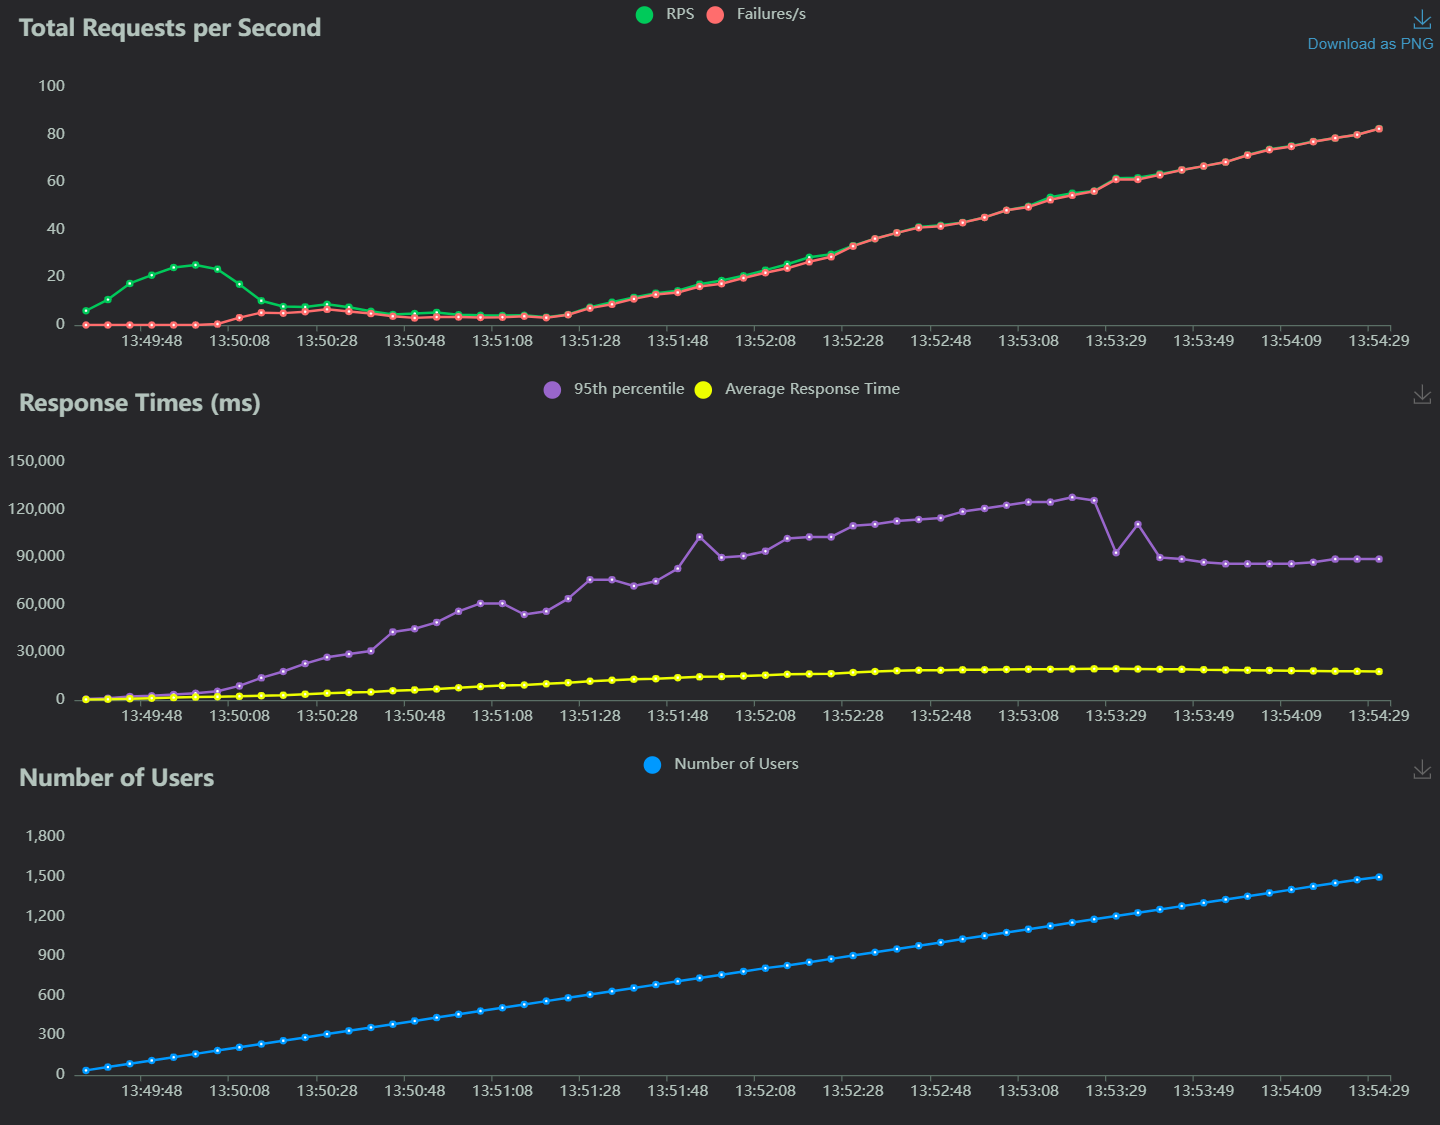
\includegraphics[width=0.87\linewidth]{fig/prueba_grafico_estadistico.png}
	\caption{Gráfico estadístico de la prueba de stress}
	\label{fig:prueba_grafico_estadistico}
\end{figure}

En la Figura \ref{fig:prueba_grafico_estadistico}, se presentan las gráficas estadísticas correspondientes a la prueba de estrés descrita.

\begin{figure}[H]
	\centering
	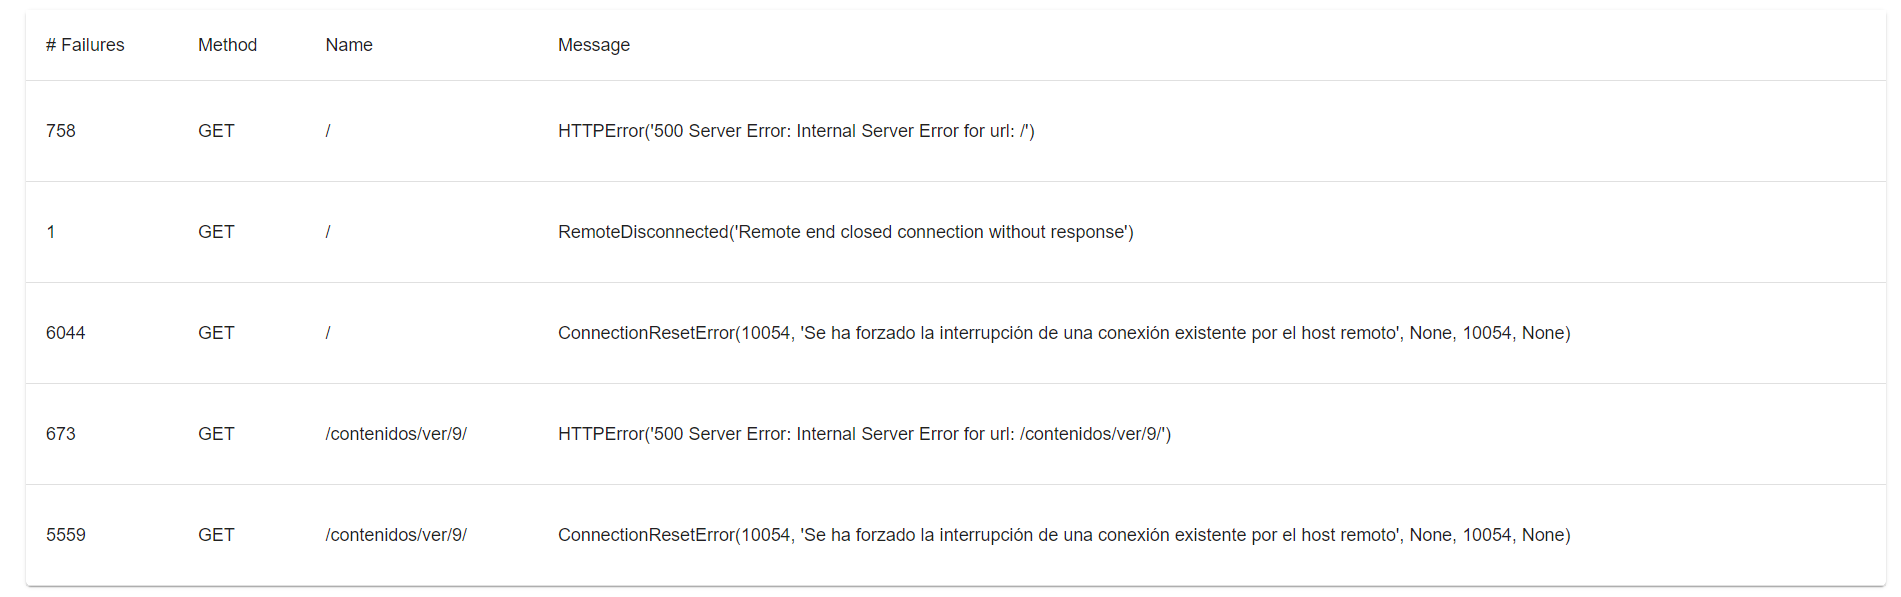
\includegraphics[width=\linewidth]{fig/prueba_errores.png}
	\caption{Errores encontrados durante la prueba de stress}
	\label{fig:prueba_errores}
\end{figure}

En la Figura \ref{fig:prueba_errores} se presentan los errores registrados durante la prueba. Profundizando un poco más, al revisar el registro del sistema, identificamos el error \textbf{FATAL:  sorry, too many clients already}, emitido por la base de datos. Este error estuvo presente desde que se detectaron los primeros problemas en las solicitudes hasta la finalización de la ejecución de la prueba.

\begin{figure}[H]
	\centering
	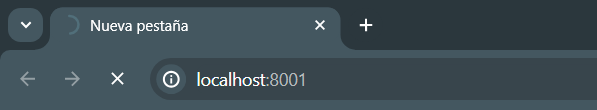
\includegraphics[width=\linewidth]{fig/prueba_sistema_caido.png}
	\caption{Sistema caído posterior a la prueba}
	\label{fig:prueba_sistema_caido}
\end{figure}

En la Figura \ref{fig:prueba_sistema_caido} se observa que finalizada la prueba de estrés, se intentó acceder nuevamente al sistema sin éxito. Esto respalda la idea de que el sistema se encontraba completamente caído.

\begin{figure}[H]
	\centering
	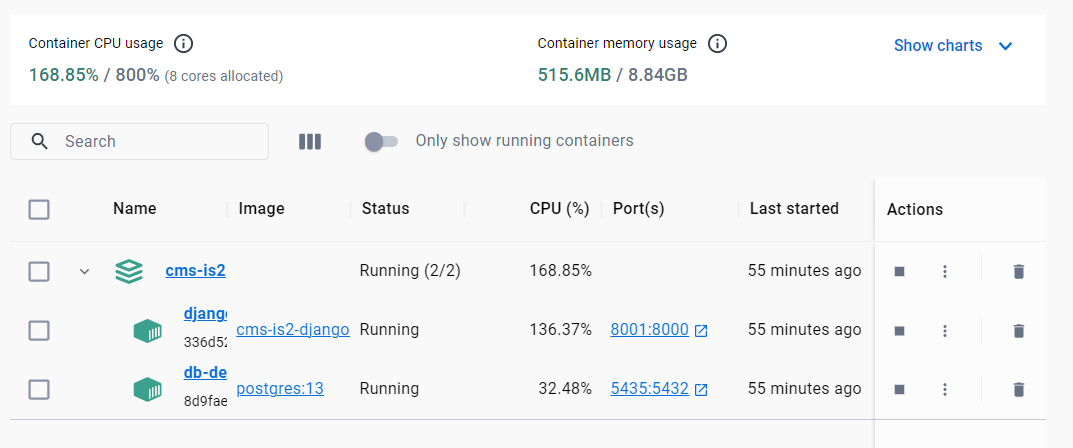
\includegraphics[width=\linewidth]{fig/docker.png}
	\caption{Uso de recursos}
	\label{fig:prueba_recursos}
\end{figure}

En la Figura \ref{fig:prueba_recursos} se muestra la utilización de los recursos disponibles del sistema. Resulta notable que no se aprovechen todos los núcleos disponibles cuando la carga es máxima.

\section{Evaluación de los casos de prueba}

En esta sección se han seleccionado cinco casos de uso para probar la funcionalidad del sistema y su capacidad de recuperación, con el fin de identificar posibles errores y evaluar su corrección y resiliencia.

\subsection{Caso 1 - Crear un contenido}
\textbf{RF-8} El sistema deberá permitir que  el autor pueda crear contenido, seleccionando una categoría.

En el Cuadro \ref{tab:caso1_esperado} se presentan los resultados para los datos esperados, mientras que en el Cuadro \ref{tab:caso1_no_esperado} los resultados para los datos no esperados.

\begin{table}[H]
    \centering
    \rowcolors{2}{gray!15}{white}
    \begin{tabular}{p{3cm}p{4cm}}
        \rowcolor{gray!15}
        Datos & Un usuario con rol de autor dentro del sistema, ingresa a la interfaz de categorias, selecciona una categoría y procede a crear un contenido. \\
       	Respuesta & Se proporcionan plantillas para los contenidos y permite al autor crear un contenido que será guardado como un borrador. \\
       	Problemas & Sin problemas. \\
       	Sugerencias & Agregar el botón de crear contenido dentro de la categoría pero fuera del apartado para el tablero kanban. \\
    \end{tabular}
    \caption{Datos esperados}
    \label{tab:caso1_esperado}
\end{table}

\begin{table}[H]
    \centering
    \rowcolors{2}{gray!15}{white}
    \begin{tabular}{p{3cm}p{4cm}}
        \rowcolor{gray!15}
        Datos & Un usuario con rol de autor dentro del sistema, ingresa a la interfaz de categorias, selecciona una categoría, selecciona el tablero kanban y procede a crear un contenido.\\
       	Problemas & Sin problemas. \\
       	Sugerencias & Agregar el botón de crear contenido dentro de la categoría pero fuera del apartado para el tablero kanban. Para crear un contenido, se debe acceder a la categoría y dentro de la categoría entrar al tablero kanban lo que puede resultar poco intuitivo.\\
    \end{tabular}
    \caption{Datos no esperados}
    \label{tab:caso1_no_esperado}
\end{table}

\subsection{Caso 2 - Inactivar un contenido}
\textbf{RF-11} El sistema permitirá que el autor inactive un contenido aunque no haya sido publicado aún.

En el Cuadro \ref{tab:caso2_esperado} se presentan los resultados para los datos esperados, mientras que en el Cuadro \ref{tab:caso2_no_esperado} los resultados para los datos no esperados.

\begin{table}[H]
    \centering
    \rowcolors{2}{gray!15}{white}
    \begin{tabular}{p{3cm}p{4cm}}
        \rowcolor{gray!15}
        Datos & Un usuario con rol de autor de un contenido entra a una categoría, selecciona un contenido de su autoría que se encuentre publicado y lo inactiva.\\
       	Respuesta & El sistema inactiva el contenido.\\
       	Problemas & Sin problemas.\\
       	Sugerencias & Sin sugerencias.\\
    \end{tabular}
    \caption{Datos esperados}
    \label{tab:caso2_esperado}
\end{table}

\begin{table}[H]
    \centering
    \rowcolors{2}{gray!15}{white}
    \begin{tabular}{p{3cm}p{4cm}}
        \rowcolor{gray!15}
        Datos & Un usuario con rol de autor de un contenido entra a una categoría, selecciona un contenido de su autoría que aún no ha sido publicado y lo inactiva.\\
        Respuesta & El sistema inactiva el contenido.\\
       	Problemas & No existe un botón o alguna instancia al que un usuario pueda acceder para inactivar un contenido que haya sido mandado para su edición y posterior revisión.\\
       	Sugerencias & Implementar un botón dentro del kanban disponible para el usuario que permita inactivar el contenido.\\
    \end{tabular}
    \caption{Datos no esperados}
    \label{tab:caso2_no_esperado}
\end{table}

\subsection{Caso 3 - Publicar un contenido}

\textbf{RF-54} El publicador de un contenido deberá definir el tiempo de vigencia del mismo, el  cual podrá ser modificado por el usuario que posea los permisos correspondientes.

En el Cuadro \ref{tab:caso3_esperado} se presentan los resultados para los datos esperados, mientras que en el Cuadro \ref{tab:caso3_no_esperado} los resultados para los datos no esperados.

\begin{table}[H]
    \centering
    \rowcolors{2}{gray!15}{white}
    \begin{tabular}{p{3cm}p{4cm}}
        \rowcolor{gray!15}
        Datos & Un usuario con rol de autor de un contenido entra a una categoría, selecciona un contenido de su autoría que se encuentre publicado y lo inactiva.\\
       	Respuesta & Habilita el contenido publicado para que los demás usuarios puedan interactuar con el.\\
       	Problemas & Sin problemas.\\
       	Sugerencias & Sin sugerencias.\\
    \end{tabular}
    \caption{Datos esperados}
    \label{tab:caso3_esperado}
\end{table}

\begin{table}[H]
    \centering
    \rowcolors{2}{gray!15}{white}
    \begin{tabular}{p{3cm}p{4cm}}
        \rowcolor{gray!15}
        Datos & Un usuario con rol de publicador procede a colocar una fecha de vigencia para el contenido posterior al día de su aprobación.\\
        Respuesta & El acepta esta fecha de vigencia. El contenido directamente pasa a estar inactivo.\\
       	Problemas & Sin Problemas.\\
       	Sugerencias & Validar la fecha de vigencia de expiración de los contenidos.\\
    \end{tabular}
    \caption{Datos no esperados}
    \label{tab:caso3_no_esperado}
\end{table}

\subsection{Caso 4 - Inactivar cuenta}

\textbf{RF-44} El usuario podrá inactivar su cuenta.

En el Cuadro \ref{tab:caso4_esperado} se presentan los resultados para los datos esperados.

\begin{table}[H]
    \centering
    \rowcolors{2}{gray!15}{white}
    \begin{tabular}{p{3cm}p{4cm}}
        \rowcolor{gray!15}
        Datos & Un usuario desea inactivar su cuenta.\\
       	Respuesta & No hay.\\
       	Problemas & No existe una opción que permita al usuario inactivar su cuenta.\\
       	Sugerencias & Agregar un apartado dentro del perfil del usuario que permita inactivar su cuenta..\\
    \end{tabular}
    \caption{Datos esperados}
    \label{tab:caso4_esperado}
\end{table}

\subsection{Caso 5 - Edición de un contenido}

\textbf{RF-61} El editor que seleccione primero lo creado por el autor será el encargado de editar ese contenido. 

En el Cuadro \ref{tab:caso5_esperado} se presentan los resultados para los datos esperados, mientras que en el Cuadro \ref{tab:caso5_no_esperado} los resultados para los datos no esperados.

\begin{table}[H]
    \centering
    \rowcolors{2}{gray!15}{white}
    \begin{tabular}{p{3cm}p{4cm}}
        \rowcolor{gray!15}
        Datos & Un usuario con rol de editor accede a una categoría, selecciona un contenido para su edición.\\
       	Respuesta & Se le permite la edición y los cambios se guardan.\\
       	Problemas & Sin problemas.\\
       	Sugerencias & Sin sugerencias.\\
    \end{tabular}
    \caption{Datos esperados}
    \label{tab:caso5_esperado}
\end{table}

\begin{table}[H]
    \centering
    \rowcolors{2}{gray!15}{white}
    \begin{tabular}{p{3cm}p{4cm}}
        \rowcolor{gray!15}
        Datos & Un segundo usuario con rol de editor accede a una categoría, selecciona un contenido que ya ha sido editado para su edición.\\
        Respuesta & Se le permite la edición y los cambios se guardan.\\
       	Problemas & El primer editor que seleccione un contenido para su edición debe ser el encargado de ese contenido para su edición.\\
       	Sugerencias & Validar los permisos de los usuarios sobre los contenidos.\\
    \end{tabular}
    \caption{Datos no esperados}
    \label{tab:caso5_no_esperado}
\end{table}
\section{Inspección de código}
\subsection{Complejidad Ciclomática}
	Utilizando la herramienta radon \cite{radon} para analizar la complejidad ciclomática. La complejidad ciclomática se mide con un número seguido de una letra que indica el nivel de complejidad:
	\begin{itemize}
		\item A (1-5): Baja complejidad
		\item B (6-10): Complejidad moderada
		\item C (11-20): Alta complejidad
		\item D (21-30): Muy alta complejidad
		\item E (31-40): Complejidad extrema
		\item F (\textgreater40): Complejidad inaceptable
		\label{itemize:rangos_compejidad}	
	\end{itemize}
	
	En el cuadro \ref{tab:tipos_complejidad}, se presenta los resultados encontrados de la cantidad de funciones o métodos agrupados según el rango\ref{itemize:rangos_compejidad} descrito anteriormente.
	
	\begin{table}[ht]
		\rowcolors{2}{gray!15}{white}
	    \begin{tabular}{ccc}
	    	\rowcolor{gray!15}
	        \textbf{Tipo} & \textbf{Cantidad} \\
	        A & 295 \\
	        B & 17 \\
	        C & 13 \\
	        D & 5 \\
	        E & 3 \\
	        F & 58 \\
	    \end{tabular}
	    \centering
	    \caption{Clasificación de complejidad por cantidad de cada tipo}
	    \label{tab:tipos_complejidad}
	\end{table}

\subsection{Métricas de linea de código y comentarios}
Para esta sección se utlizaron las siguientes métricas:
\begin{itemize}
\item\textbf{Archivos totales:} Indica la cantidad total de archivos analizados.
\item\textbf{Total de líneas de código (LOC):} Es la suma total de todas las líneas de código encontradas en los archivos. Es el número total de líneas de código en bruto, incluyendo comentarios y líneas en blanco.
\item\textbf{Total de líneas de código legibles (LLOC):} Representa las líneas de código que contienen contenido real o legible del programa. Generalmente excluye comentarios y líneas en blanco.
\item\textbf{Total de líneas de código fuente (SLOC):} Similar a LLOC, pero podría incluir líneas de código generadas automáticamente (por ejemplo, por herramientas o plantillas), además del código escrito a mano.
\item\textbf{Total de líneas de comentarios de línea única:} Indica la cantidad de líneas que contienen comentarios en una sola línea.
\item\textbf{Total de líneas de comentarios de múltiples líneas:} Representa la cantidad de líneas que contienen comentarios que ocupan varias líneas.
\end{itemize}

 En la siguiente tabla \ref{tab:cantidad_LDC_Comentarios} , se presentan los resultados obtenidos que reflejan estas métricas de análisis de código.


	\begin{table}[ht]
		\rowcolors{2}{gray!15}{white}
	    \begin{tabular}{ccc}
	    	\rowcolor{gray!15}
	        \textbf{Tipo} & \textbf{Cantidad} \\
	        Archivos totales & 73 \\
	        Líneas de código totales(LOC) & 3487 \\
	        Líneas de código lógicas(LLOC) & 1644 \\
	        Líneas de código fuente(SLOC) & 1831 \\
	        Cantidad de comentarios de línea única  & 219 \\
	        Cantidad de comentarios de múltiples líneas & 686 \\
                  Cantidad de líneas en blanco & 750\\
	    \end{tabular}
	    \centering
	    \caption{Clasificación de complejidad por cantidad de cada tipo}
	    \label{tab:cantidad_LDC_Comentarios}
	\end{table}

\section{Conclusiones}
Las pruebas de software desempeñan un papel fundamental en el desarrollo del Sistema de Gestión de Contenidos, garantizando no solo la detección y corrección de errores, sino también la evaluación exhaustiva de la funcionalidad para asegurar la calidad del sistema. \newline
El proyecto se ha centrado en la implementación de diversos tipos de pruebas y técnicas especializadas para cumplir con los estándares esperados. Se han utilizado pruebas de diferentes escenarios, desde casos de uso típicos hasta situaciones específicas, asegurando así la fiabilidad y consistencia del software. \newline
Además de las pruebas estándar, se han aplicado técnicas como las pruebas de interfaz gráfica para validar la usabilidad y el diseño visual, y las pruebas de estrés para evaluar la estabilidad y capacidad de respuesta bajo condiciones extremas. La verificación del modelo de datos ha sido crucial para asegurar la integridad de la estructura de datos y prevenir errores que puedan comprometer la información. \newline
El equipo de pruebas ha seguido una metodología bien definida que incluyó desde el contacto inicial con los responsables del sistema hasta la planificación detallada de actividades y la ejecución meticulosa de las pruebas. \newline
Durante la ejecución, se documentaron los hallazgos obtenidos en cada fase de las pruebas, garantizando una recopilación precisa y oportuna de los resultados y observaciones relevantes. Finalmente, en una reunión final se revisaron y discutieron los hallazgos, sacando conclusiones e identificando lecciones aprendidas.

\printbibliography

\end{document}

